\newpage
\hypertarget{common cspConstraint}{}
\subsection{Implementing SetDefaultNumber}
\genHeader

We've declared and used our custom \texttt{SetDefaultNumber} constraint, but we haven't given it any implementation code yet. If you haven't yet, save and build
\texttt{DictionaryCodeAdapter} before continuing.

\begin{itemize}

\item[$\blacktriangleright$] Navigate to ``/src,'' where a new \texttt{csp.constraints} package was generated, and open \texttt{SetDefaultNumber.java}. Edit
this file until it matches Fig.~\ref{eclipse:setDefaultImpl}.

\begin{figure}[htbp]
\begin{center}
  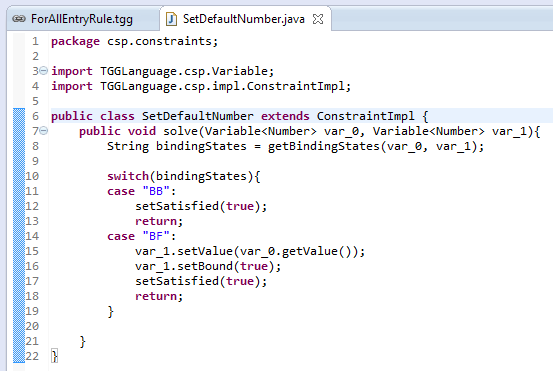
\includegraphics[width=0.9\textwidth]{eclipse_setDefaultNumberImplementation}
  \caption{extra constraint impl}
  \label{eclipse:setDefaultImpl}
\end{center}
\end{figure}

\item[$\blacktriangleright$] Save, build, and run \texttt{TGGMain} one more time. The inital and final \texttt{tree} variants should now be nearly identical! If
you're worried about some of the nodes being in the wrong order (such as an author at the bottom of the list), double-click on them and check their
\texttt{index} properties. If everything has been done correctly every \texttt{entry} should be 2, each \texttt{author} should be 1, and each \texttt{title}
should be 0.

\item[$\blacktriangleright$] On a final note to end the model-to-text step, wasn't it great how easy and short this was? If we were to use another
transformation set up (such as SDMs), we would have had to create independent rules for this backwards direction. Instead, TGGs gave us this transform for free!

\end{itemize}
